\subsection{Intensity of Attraction}

Asymptotic resilience notably relies on linearizing at a point attractor. In contrast, intensity of attraction, originally introduced by Richard McGehee for discrete maps \cite{mcgeheeMetricPropertiesAttractors1988}, and extended to the continuous case by Katherine Meyer \cite{meyerMetricPropertiesAttractors2019}, measures resilience not only for rest points but also for any other type of attractor. Even more importantly, it captures metric information across the entire basin of attraction rather than simplifying to a topologically equivalent approximation within a limited neighborhood. We now review the necessary background in order to define intensity of attraction. 

First of all, the idea of perturbation will now be represented by what is known as a \textbf{control function} added to an underlying vector field. This construction allows for perturbations which are not necessarily small and isolated, but possibly large and continuous, reflecting important types of perturbation that commonly occur in ecological and other applied settings, such as environmental forces or human-driven pressure (intentional or unintentional) on an ecosystem. We assume that the control function $$g: I \subset \mathbb{R} \to \mathbb{R}^n$$ is taken from the space of essentially bounded (i.e. bounded except on a set of measure 0) measurable functions $L^\infty (I,\mathbb{R}^n)$, where the norm is 
$$||g||_\infty = \inf\{C \geq 0  :  ||g(x)|| \leq C  \text{ for almost every } x \in I \}.$$ 
%These mild assumptions will ensure that $g$ is nice enough for our perturbed system to remain well-defined. 
Next, we formalize how the perturbation is added to an underlying system. 

\begin{definition}
	A \textbf{bounded control system} is a non-autonomous ODE 
	\begin{equation}
		\label{eqn:control_ode}x' = f(x) + g(t)
	\end{equation}
	where $f: U \subset \mathbb{R}^n \to \mathbb{R}^n$ is locally Lipschitz, $g \in L^\infty (I,\mathbb{R}^n)$. \qed
\end{definition}

Here, the underlying system is thought of as an ODE $x'=f(x)$; but it is altered by adding a perturbation $g(t)$ to the vector field $f(x)$ on the right hand side. The effect of $g(t)$ is to adjust, at every point in time, the path of solutions somewhat away from what would have been their original trajectory. 

It remains to be justified whether this construction produces a well-defined system. Because the right hand side $f(x) + g(t)$ may be a discontinuous function, solutions $x(t)$ of the ODE must be considered in an extended sense, which is that $x'(t) = f(x) + g(t) \text{ almost everywhere.}$ Fortunately, the conditions on $g$ are enough to guarantee local existence and uniqueness of solutions in such an extended sense. Briefly: (1) the hypotheses of Carath\'eodory's theorem are satisfied, establishing existence, and (2) boundedness of $g$ guarantees Lipschitz continuity (local if $f$ is locally Lipschitz, global if $f$ is globally Lipschitz), thereby implying uniqueness. 

So we have well-defined solutions, and can therefore extend the standard local flow notation to the bounded control setting. Fixing an underlying vector field $f$, we will denote as follows the flow obtained by applying a choice of perturbation $g$.

\begin{definition} 
	$\varphi_g(t, x_0): D \subset \mathbb{R} \times U \to U$ is the local flow defined by $$\varphi_g(t, x_0) = x(t)$$ where $x(t)$ solves in the extended sense the ODE (\ref{eqn:control_ode}), with initial condition $x(0) = x_0$. \qed
\end{definition}

Intensity of attraction considers not just one single control function, but entire families of control functions -- specifically, those where every function is bounded by some maximum magnitude $r$. %Supposing that vector field perturbations are limited by some ceiling $r$ on magnitude, each family can be thought of as a collection of all possible perturbations. 
The next definition gives a notation for these families.


\begin{definition}
	Denote by $B_r \subset L^\infty[I, \mathbb{R}^n]$ the set of control functions bounded above by $r$:
	$$B_r = \{g  : ||g||_\infty < r\}$$ \qed
\end{definition}

%Then, again fixing an underlying vector field $f$, the collection of all possible perturbed trajectories can be captured by the following notation.

%\begin{definition} 
%	\begin{align*}
%		\Psi_{r} = \{ 
%		(a, b, T) : ~&\exists
%		\text{ a control function } 
%		g \in B_r \text{ such that some solution } x:[0,T] \to \mathbb{R}\\
%		& \text{ of the associated bounded control system }
%		x' = f(x) + g(t)\\
%		& \text{ has endpoints }
%		x(0) = a, x(T) = b
%		\}
%	\end{align*} \qed
%\end{definition}

This leads, next, into the notion of all possible states reachable in forward time, under the family of all possible control functions bounded by $r$, and beginning from some arbitrary initial set of states.  

\begin{definition}
	Consider $S\subset  U$. The \textbf{reachable set} of $S$ under $r$-bounded control is the set
	$$R_r(S) =  \bigcup\limits_{g \in B_r} \bigcup\limits_{x_0 \in S} \bigcup\limits_{t \geq 0}  \varphi_g(t,x_0)$$ \qed
\end{definition}

Finally, we are ready to define intensity of attraction, which captures the folllowing idea: what is the smallest magnitude of control necessary in order to escape from (all compact subsets of) a basin of attraction?

\begin{definition}
	If $A$ is an attractor of $x' = f(x)$, then its \textbf{intensity of attraction} is 
	$$intensity(A) = \sup\{ r \geq 0 ~|~ R_r(A) \subset K \subset basin(A), \text{ for some compact }K \}$$ \qed
\end{definition}
	
\begin{example}
A predator-prey model (Figure \ref{fig:predator_prey_reachable_sets}). 

\begin{figure}[H]
\centering
\captionsetup{width=0.9\linewidth}
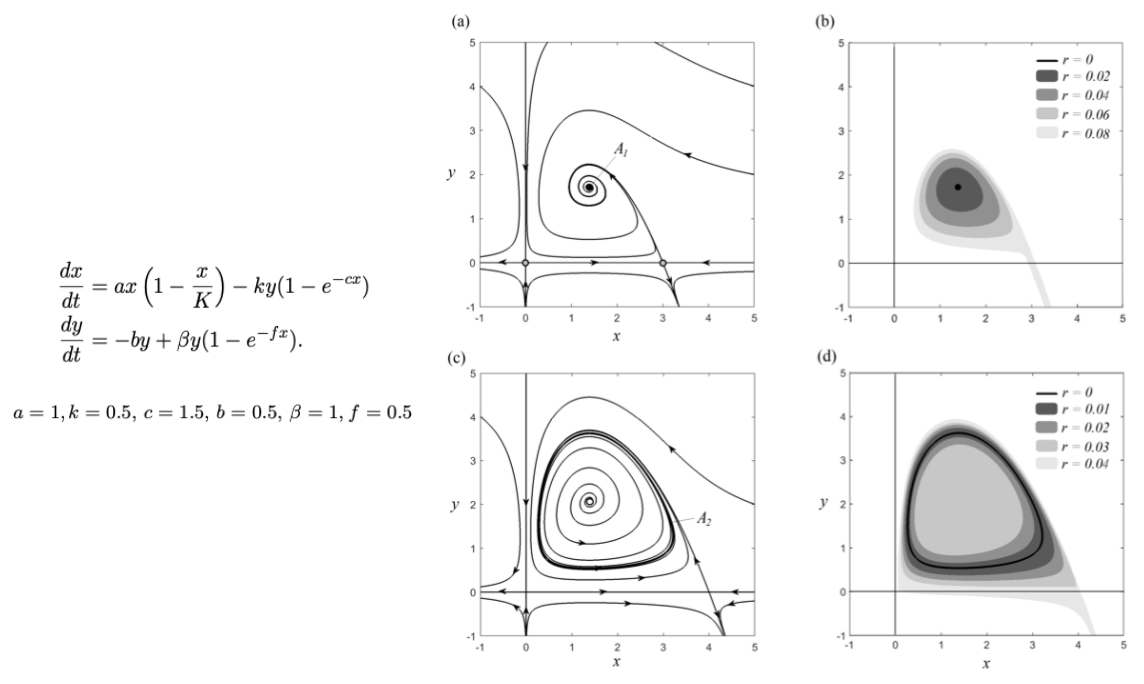
\includegraphics[width=\textwidth]{figs/predator_prey_reachable_sets} 
\caption{
	(a) phase portrait with parameter choice $K = 3$. (b) numerical computation of reachable sets shows that the intensity of the point attractor $A_1$ is between $0.06$ and $0.08$. (c) phase portrait with parameter choice $K=4$. (d) numerical computation of reachable sets shows that the intensity of the periodic attractor $A_2$ has intensity between $0.03$ and $0.04$. Figure reproduced from \cite{meyerMetricPropertiesAttractors2019}.}\qed
\label{fig:predator_prey_reachable_sets}
\end{figure}
\end{example}

Another way to understand intensity of attraction is through the idea of "basin steepness" -- what is the steepest part of the basin that must be overcome in order to escape the influence of the attractor? For systems whose state $x$ is one dimensional, this intuition is precise: the vector field $f: \mathbb{R} \to \mathbb{R}$ is always integrable, producing a potential function, and the maximum steepness of that potential on the basin determines intensity of attraction.
%
%\begin{proposition}
%	To do: 1D basin steepness
%\end{proposition}
%
%\begin{proof}
%	content...
%\end{proof}
%
%Add figure with 1D example
%
Unfortunately, for two and higher dimensional systems, no potential function necessarily exists, complicating the landscape analogy. Still, the next conjecture formalizes a sense in which intensity equals basin steepness. This conjecture has not yet been proven, but in McGehee's original conception of intensity for discrete maps, an analogous statement is true. %\todo{cite personal communication with Kate}

\begin{conjecture}
	\label{conj:steepness}
	If there is a neighborhood $N$ of the attractor whose closure is within its basin of attraction, such that the inward normal component of the vector field $f$ at every point on the boundary of $N$ is at least $k$, then the intensity of the attractor is at least $k$.
\end{conjecture}

%Add picture

%Add example of intensity changing while asymptotic resilience does not change. 